\documentclass[conference]{IEEEtran}
\usepackage{cite}
\usepackage{amsmath,amssymb,amsfonts}
\usepackage{graphicx}
\usepackage{booktabs}
\usepackage{multirow}
\usepackage{url}
\usepackage{hyperref}
\graphicspath{{figures/}}

\begin{document}

\title{AICD: An Auditable Study of Label Provenance, Explanation Faithfulness, and Distribution Shift in RTL Gate-Count Estimation}

% Replace the author block before submission.
\author{\IEEEauthorblockN{Author Name 1, Author Name 2}
\IEEEauthorblockA{Department / Institution\\City, Country\\email@institution.edu}}

\maketitle

\begin{abstract}
Machine-learning estimators can provide early feedback on RTL designs without running a complete synthesis flow, but their reliability depends on feature coverage, label provenance, and distribution shift. This paper presents AICHD, an auditable framework that extracts 24 lightweight source-level features, trains a default Random Forest estimator, compares alternative regressors, and exposes predictions through an interactive inference workbench. The research pipeline generates 500 RTL modules, obtains synthesis-derived labels with Yosys when selected, computes TreeSHAP and permutation explanations, and compares their rankings with mean-replacement ablation. A zero-shot evaluation on 17 open-source RTL modules obtains $R^2=-0.068$ and MAE 8,218.69 gates, demonstrating that strong in-distribution results do not imply production-scale generalization. Explanation agreement is reported as a protocol-dependent empirical diagnostic rather than a guarantee of causal faithfulness. The workbench additionally proposes RTL rewrites but exposes corrected code only after formal equivalence checking, exhaustive simulation for eligible small combinational designs, and a measured reduction in synthesized cell count or logic depth; failed, ambiguous, or unsupported cases are withheld with diagnostics. In a controlled benchmark, batch ML inference is 423.2$\times$ faster than the measured Yosys synthesis path. The resulting contribution is an auditable workflow for lightweight RTL estimation, explanation, and verification-aware optimization, together with explicit evidence about its current limitations.
\end{abstract}

\begin{IEEEkeywords}
RTL estimation, logic synthesis, gate count, explainable AI, SHAP, distribution shift, electronic design automation.
\end{IEEEkeywords}

\section{Introduction}

Register-transfer-level (RTL) design is an important point at which architectural and implementation decisions can still be changed at relatively low cost. However, accurate area or gate-count feedback usually requires downstream elaboration and synthesis. The resulting latency complicates design-space exploration, particularly when many modules or parameter settings must be evaluated. Machine-learning (ML) methods have therefore been studied as inexpensive proxies for presynthesis power, performance, and area (PPA) estimation. Recent systems include graph representations of RTL and netlists, transfer learning across tool settings, data augmentation, and graph-convolutional design-space optimization methods \cite{fang2023masterrtl,fang2025transfer,francisco2021ppa,levy2024fastpase}.

The central difficulty addressed in this paper is not simply predictive accuracy. An estimator can obtain a high score on a synthetic test split while learning a relationship specific to the data generator or label-construction procedure. Similarly, a feature-attribution method can produce plausible explanations without demonstrating that its ranking tracks the model's actual sensitivity. These problems are especially important in electronic design automation (EDA), where labels may depend on synthesis scripts, hierarchy treatment, libraries, and timeout policies.

AICD is designed as an auditable framework for studying these effects in RTL gate-count estimation. The framework extracts a small set of source-level features, trains lightweight regression models, records provenance for generator and synthesis-derived labels, computes explanation rankings, and evaluates zero-shot behavior on open-source RTL. The paper makes four contributions:
\begin{enumerate}
\item We define a reproducible label-provenance protocol that evaluates the same feature table under generator-derived, regex/default, and Yosys-derived gate-count targets.
\item We report repeated-seed performance rather than relying on a single favorable split, showing how label choice changes both accuracy and error scale.
\item We evaluate zero-shot transfer to real RTL and report the distribution-shift failure modes, including hierarchy-heavy and memory-dominated modules.
\item We synchronize SHAP, permutation importance, and ablation on one held-out set, providing an empirical check of explanation rankings while explicitly discussing the limitations of mean-replacement perturbations.
\end{enumerate}

The intended claim is deliberately narrower than a new state-of-the-art PPA predictor. AICD contributes an auditable methodology and a failure analysis for lightweight RTL gate-count estimators. This positioning distinguishes the work from prior systems that primarily optimize predictive accuracy or transferability \cite{fang2023masterrtl,fang2025transfer,chattopadhyay2025ppa}.

\begin{figure*}[t]
\centering
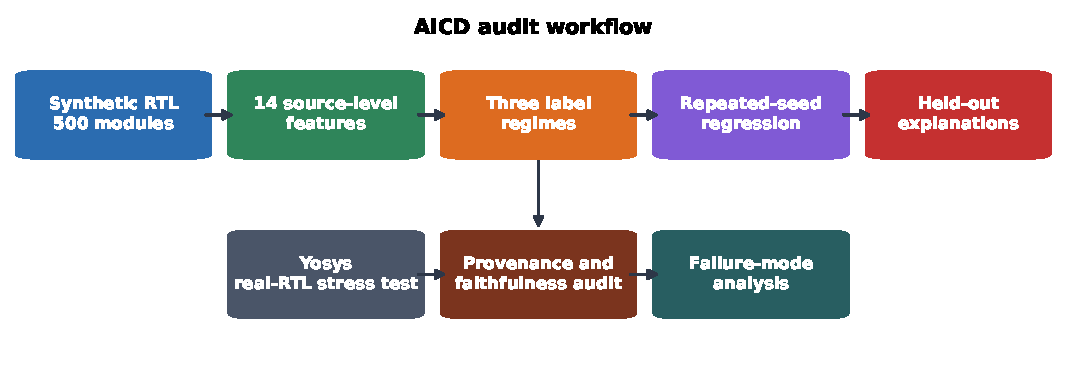
\includegraphics[width=\textwidth]{workflow}
\caption{AICD's auditable workflow. The same extracted feature representation is evaluated under multiple label regimes, repeated splits, held-out explanation checks, and a zero-shot real-RTL stress test.}
\label{fig:workflow}
\end{figure*}

\section{Related Work}

\subsection{Presynthesis PPA estimation}
MasterRTL converts HDL into a bit-level Simple Operator Graph (SOG) to reduce the representation gap between RTL and gate-level structure. Its ICCAD paper evaluates timing, power, and area on a broad design collection and reports improvements over prior methods \cite{fang2023masterrtl}. A subsequent IEEE TCAD article adds graph- and LLM-based data augmentation and studies transfer across designs, technology nodes, and process corners \cite{fang2025transfer}. FastPASE instead uses graph convolutions on elaborated RTL dataflow graphs and demonstrates faster design-space optimization for SIMD and RISC-V case studies \cite{levy2024fastpase}. Transfer-learning-based PPA modeling studies the impact of synthesis and place-and-route recipes on early prediction \cite{francisco2021ppa}. Recent SOG-based work also reports early WNS, TNS, and power estimation on 147 RTL designs \cite{chattopadhyay2025ppa}.

These papers establish that presynthesis estimation is an active and competitive research area. AICD therefore does not claim novelty for using ML to estimate RTL metrics. Instead, it focuses on the audit questions that arise when a lightweight estimator is evaluated: which labels were used, how stable are results across splits, how far does a syntactic model transfer to real RTL, and do explanation rankings agree with measured model sensitivity?

\subsection{Feature attribution and faithfulness}
SHAP provides a unified additive attribution framework with theoretical properties for assigning feature contributions to individual predictions \cite{lundberg2017shap}. Permutation importance measures the change in a performance metric after a feature is perturbed, but correlated features and unrealistic perturbations can alter its interpretation \cite{altmann2010permutation}. More generally, faithfulness evaluations are protocol-dependent: an attribution is useful only relative to a defined intervention and evaluation distribution. AICD treats faithfulness as an empirical property to be measured for this RTL feature space, not as an automatic consequence of applying SHAP.

\section{Auditable Methodology}

\subsection{Feature representation}
Each Verilog module is represented using 14 source-level features. Structural features count inputs, outputs, wires, and instances. Operator features count AND, OR, XOR, NOT, NAND, and NOR occurrences. Complexity features count nonempty lines and characters, while bitwidth features record average and maximum declared widths. The representation is intentionally lightweight and does not require a full elaborated netlist or technology library.

\subsection{Label provenance}
AICD stores three possible label regimes. The generator regime uses the gate-count file emitted together with the synthetic RTL. The regex/default regime uses the repository's default label file. The synthesis regime runs Yosys and records primitive-cell counts using a documented synthesis script. All label tables are normalized to a numeric module identifier before joining with the feature table. This normalization is essential because the feature file uses identifiers such as \texttt{rtl\_module\_0}, whereas label files use numeric identifiers.

The distinction is scientifically important. The default collector gives priority to generator ground truth when it is present, then uses Yosys, and finally falls back to regex counting. Consequently, the phrase ``Yosys ground truth'' is reserved in this paper for experiments that explicitly use the Yosys label table.

\begin{figure}[t]
\centering
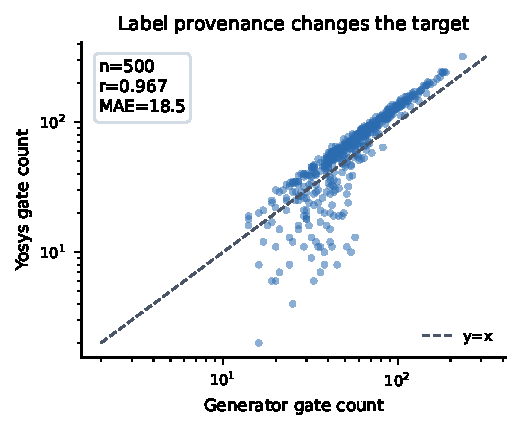
\includegraphics[width=\columnwidth]{label_provenance}
\caption{Generator and Yosys gate-count labels for the 500 common synthetic modules. The high rank correlation does not imply identical absolute targets.}
\label{fig:label-provenance}
\end{figure}

\subsection{Predictive models and repeated evaluation}
We compare linear regression and a Random Forest regressor. The Forest uses 100 trees in the repeated evaluation, maximum depth 20, minimum split size 5, minimum leaf size 2, and fixed model seed 42. For each label regime, 10 independent train/test splits are generated with test fraction 15\%. The same split seeds are used for every regime and model. We report the mean, standard deviation, minimum, and maximum of $R^2$, MAE, and RMSE across seeds.

\subsection{Explanation-faithfulness protocol}
For one synchronized generator-label experiment, the Forest is trained on the training subset. On the held-out subset, we compute (i) mean absolute TreeSHAP values, (ii) permutation importance using 30 repeats and negative MAE scoring, and (iii) single-feature mean-replacement ablation. The ablation score for feature $j$ is
\begin{equation}
\Delta_j = \operatorname{MAE}(f(X_{\setminus j}, \bar{x}_{j,\mathrm{train}})) - \operatorname{MAE}(f(X)),
\end{equation}
where the replacement value is computed from the training subset only. We compare rankings using Spearman correlation, Kendall's $\tau$, and top-$k$ overlap. Because mean replacement can produce combinations that are rare or impossible in the original RTL distribution, this protocol is interpreted as a controlled diagnostic rather than an absolute proof of causal importance.

\subsection{Real-RTL stress test}
The zero-shot benchmark contains 20 public Verilog modules from UART, I2C, and AXI-Stream repositories. Seventeen modules complete synthesis within the timeout and are included in the primary metrics; three are reported as exclusions. Yosys counts are hierarchy-inclusive and are produced without a technology-library mapping. We report raw gate-count metrics and inspect extreme modules separately.

\section{Experimental Results}

\subsection{Repeated-seed accuracy}
Table~\ref{tab:accuracy} summarizes the clean repeated-seed evaluation. Generator and regex/default labels are identical in the current frozen artifact, while Yosys labels span a different count range and are more difficult to predict. Linear regression is the strongest model under all regimes in this feature space, indicating that the synthetic generator encodes an approximately linear relationship between feature counts and labels. This should not be interpreted as evidence that real RTL gate count is generally linear.

\begin{table}[t]
\centering
\caption{Repeated-seed test performance over 10 random 85/15 splits. Values are mean $\pm$ standard deviation.}
\label{tab:accuracy}
\small
\begin{tabular}{@{}llrr@{}}
\toprule
Label regime & Model & $R^2$ & MAE (gates)\\
\midrule
Generator & Linear regression & $0.9978\pm0.0004$ & $1.17\pm0.09$\\
Generator & Random Forest & $0.9735\pm0.0106$ & $3.73\pm0.61$\\
Yosys & Linear regression & $0.9565\pm0.0106$ & $7.24\pm0.57$\\
Yosys & Random Forest & $0.9313\pm0.0121$ & $9.27\pm0.96$\\
\bottomrule
\end{tabular}
\end{table}

\begin{figure}[t]
\centering
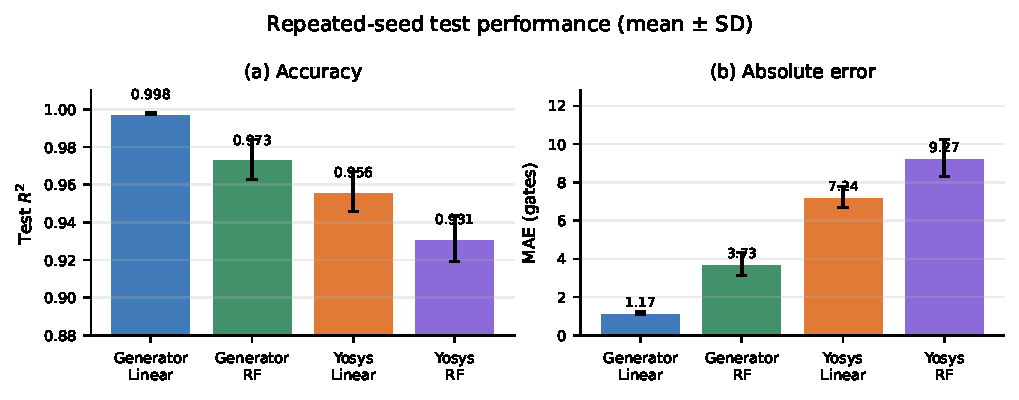
\includegraphics[width=\columnwidth]{repeated_seed_accuracy}
\caption{Repeated-seed test performance. Error bars denote standard deviation across ten held-out splits. Yosys-derived targets are more difficult than generator-derived targets for the same source-level representation.}
\label{fig:repeated-seed}
\end{figure}

Across 500 common modules, generator and Yosys labels have Pearson correlation $r=0.9666$, Spearman correlation $\rho=0.9396$, and mean absolute difference 18.534 gates. Thus, the label regimes preserve much of the ordering while changing the absolute target. This explains why a model can perform well on generator labels while suffering a measurable accuracy drop on synthesis-derived labels.

\subsection{Explanation faithfulness}
On the synchronized generator-label held-out set, the Random Forest's base MAE is 5.20 gates. SHAP and permutation rankings each obtain Spearman $\rho=1.00$ and Kendall $\tau=1.00$ against mean-replacement ablation; both have top-5 overlap 5/5. The leading features are character count, NOR count, NAND count, XOR count, and NOT count. The result indicates that, under this controlled feature space and perturbation protocol, the attribution rankings track the measured model sensitivity.

The result must be interpreted carefully. The evaluation is model- and distribution-specific, and perfect rank agreement does not establish causal importance or robustness under correlated, conditional, or retraining-based interventions. The revised artifact should repeat this analysis across seeds and for the Yosys-label model before final submission.

\begin{figure}[t]
\centering
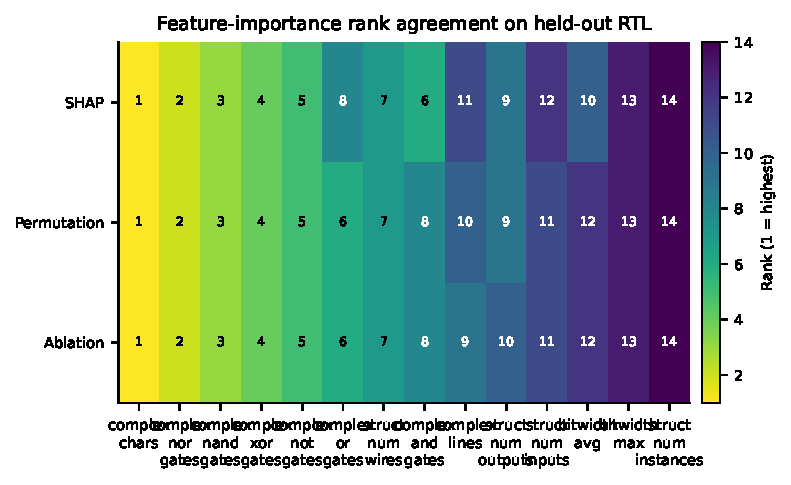
\includegraphics[width=\columnwidth]{xai_rank_agreement}
\caption{Feature-importance ranks for SHAP, permutation importance, and mean-replacement ablation on the synchronized held-out set. Lower rank numbers indicate higher importance.}
\label{fig:xai-ranks}
\end{figure}

\subsection{Zero-shot real-RTL behavior}
The real-RTL stress test obtains $R^2=-0.0685$ and MAE 8,218.69 gates on 17 successfully synthesized modules. Actual counts range from 7 to 133,594 gates, whereas predictions cluster near the center of the synthetic training distribution. The largest discrepancy is \texttt{axis\_fifo}, whose hierarchy-inclusive count is 133,594 under the stated Yosys policy. Smaller flat modules such as \texttt{axis\_register} are substantially easier than hierarchy-heavy or memory-dominated designs.

This result is a central finding rather than an embarrassment to hide. It demonstrates that strong in-distribution metrics do not imply transfer to production-scale RTL when the training distribution lacks memories, deep hierarchy, parameterized structures, and wider count ranges.

\begin{figure}[t]
\centering
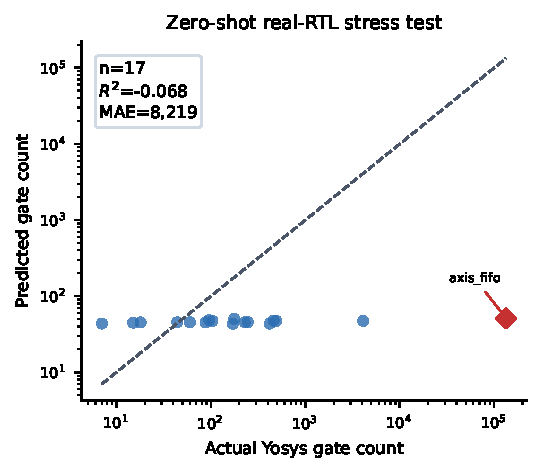
\includegraphics[width=\columnwidth]{real_rtl_shift}
\caption{Zero-shot transfer to 17 real RTL modules. Log axes expose the large count range and the concentration of predictions near the synthetic training distribution.}
\label{fig:real-rtl-shift}
\end{figure}

\section{Discussion}

AICD yields three practical conclusions. First, label provenance changes the scientific meaning of an accuracy number. Generator-derived labels can be useful for controlled methodological studies, but they should not be described as synthesis ground truth. Second, source-level features can capture simple structural regularities at very low cost, but the same representation lacks the dynamic range and semantic information needed for robust zero-shot generalization. Third, explanation methods should be evaluated against a declared intervention protocol. Agreement between SHAP, permutation, and ablation is evidence about this model and protocol; it is not a universal guarantee.

The study has several limitations. The synthetic corpus contains only 500 modules and lacks a broad family-level split. The real benchmark is drawn from a narrow set of open-source repositories, and three modules fail the synthesis timeout. Yosys counts without a technology library are useful reproducible targets but are not equivalent to a commercial standard-cell area metric. The current explanation experiment uses mean replacement and must be complemented by conditional or retraining-based ablation. Finally, the paper's numerical tables are tied to a frozen artifact snapshot; all files, seeds, software versions, synthesis scripts, and source commits must be released together.

\section{Conclusion}

This paper presented AICD, an auditable framework for lightweight RTL gate-count estimation. By separating generator and Yosys label provenance, repeating evaluation across seeds, measuring zero-shot real-RTL behavior, and checking explanations against ablation, the study exposes a pattern that raw test accuracy alone would hide: simple synthetic targets are easy to predict, synthesis-derived targets are harder, and real RTL produces substantial distribution shift. The main research value is therefore methodological and diagnostic. Future work should expand the corpus, add family-aware splits and diverse repositories, model hierarchy and memory explicitly, and evaluate explanation faithfulness under conditional interventions.

\bibliographystyle{IEEEtran}
\bibliography{refs_revised}
\end{document}
